% AVR Multi Motor Control - Paolo Lucchesi
% Slides for project presentation
\documentclass{beamer}
\usepackage[T1]{fontenc}
\usepackage[utf8]{inputenc}
\usepackage{longtable,booktabs,array}
\usepackage{caption}
\usepackage{adjustbox}
\usepackage{palatino}

\newcommand*{\LimitedIncludeGraphics}[2][]{%
\begin{adjustbox}{max size={\textwidth}{\textheight}}
    \includegraphics[#1]{#2}%
\end{adjustbox}
}

\usetheme[]{Berlin}
\usecolortheme{beaver}
\beamertemplatenavigationsymbolsempty

\hypersetup{
  pdfauthor={Paolo Lucchesi},
  hidelinks
}


\title{AVR Multi Motor Control}
\author{Paolo Lucchesi}
\date{}

\begin{document}
\frame{\titlepage}

\hypertarget{introduction}{%
\section{Introduction}\label{introduction}}

\begin{frame}{What is ammc?}
\emph{AVR Multi Motor Control} is an electrical motor management
hardware/software ecosystem composed of:

\begin{itemize}
  \item A text-based \textbf{client} application
  \item One \textbf{master} controller
  \item One or more \textbf{slave} controllers
\end{itemize}
\end{frame}

\begin{frame}{Features}
\begin{itemize}
  \item Text-based client application for POSIX environments
  \item Master and Slave(s) controller firmware
  \item Fully binary Client-Master communication protocol on top of the serial
    interface
  \item Fully binary Master-Slave communication protocol on top of the I2C
    interface
  \item Up to 126 DC motors (limited by 7-bit I2C Slave addressing, 0x00 is
    reserved)
  \item Ability to get and set the DC motors speed, individually
  \item Software defined PID controller embedded in each Slave controller
\end{itemize}
\end{frame}

\begin{frame}{Development}
\begin{itemize}
  \item Focus on \textbf{modularity}
  \item Keeping \emph{SOLID} principles in mind
  \begin{itemize}
    \item Extensibility through the Open-Close Principle
    \item Attention on module call directions following the Single
      Responsability Principle
  \end{itemize}
  \item Exhaustive \textbf{documentation} on multiple depths
  \begin{itemize}
    \item README.md file in the git repository
    \item Source code documentation generated with \emph{doxygen}
    \item Client application's man page
    \item Bachelor degree thesis
  \end{itemize}
  \item GNU Make build system
  \item Absence of third-party non-standard libraries
\end{itemize}
\end{frame}

\hypertarget{client-application}{%
\section{Client Application}\label{client-application}}

\begin{frame}{Features}
\begin{itemize}
  \item Granular handling for getting and setting motors' speed
  \item Terminal User Interface implemented as a command shell
  \item Support for non-interactive use (i.e.~scripting)
  \item Communication with master controller using the serial protocol
  \item Compatible with POSIX-compliant environments
  \item Comes with a man page
\end{itemize}
\end{frame}

\begin{frame}{Software modules}
\begin{figure}
  \centering
  \LimitedIncludeGraphics{../source/images/client-deps.png}
  \caption{Client application modules dependency graph}
\end{figure}
\end{frame}

\begin{frame}{User Interface}
External commands allow to interface the master controller:

\begin{itemize}
  \item \texttt{connect\ \textless{}device-path\textgreater{}}
  \item \texttt{ping\ \textless{}motor-id\textgreater{}}
  \item \texttt{get-speed\ \textless{}motor-id\textgreater{}}
  \item \texttt{set-speed\ \textless{}motor-id\textgreater{}=\textless{}speed\textgreater{}}
  \item \texttt{apply}
  \item \texttt{set-slave-addr}
\end{itemize}
\end{frame}

\hypertarget{master-controller}{%
\section{Master Controller}\label{master-controller}}

\begin{frame}{Features}
\begin{itemize}
  \item Is itself an \textbf{ATMega2560} microcontroller unit
  \item Interfaces the client applications with the slave controllers
  \item Communicates with the client via serial
  \item Communicates with slaves via I2C
  \item Interrupt-driven communication
  \item Comes with a power saving policy
\end{itemize}
\end{frame}

\begin{frame}{Hardware setup}
\begin{figure}
  \centering
  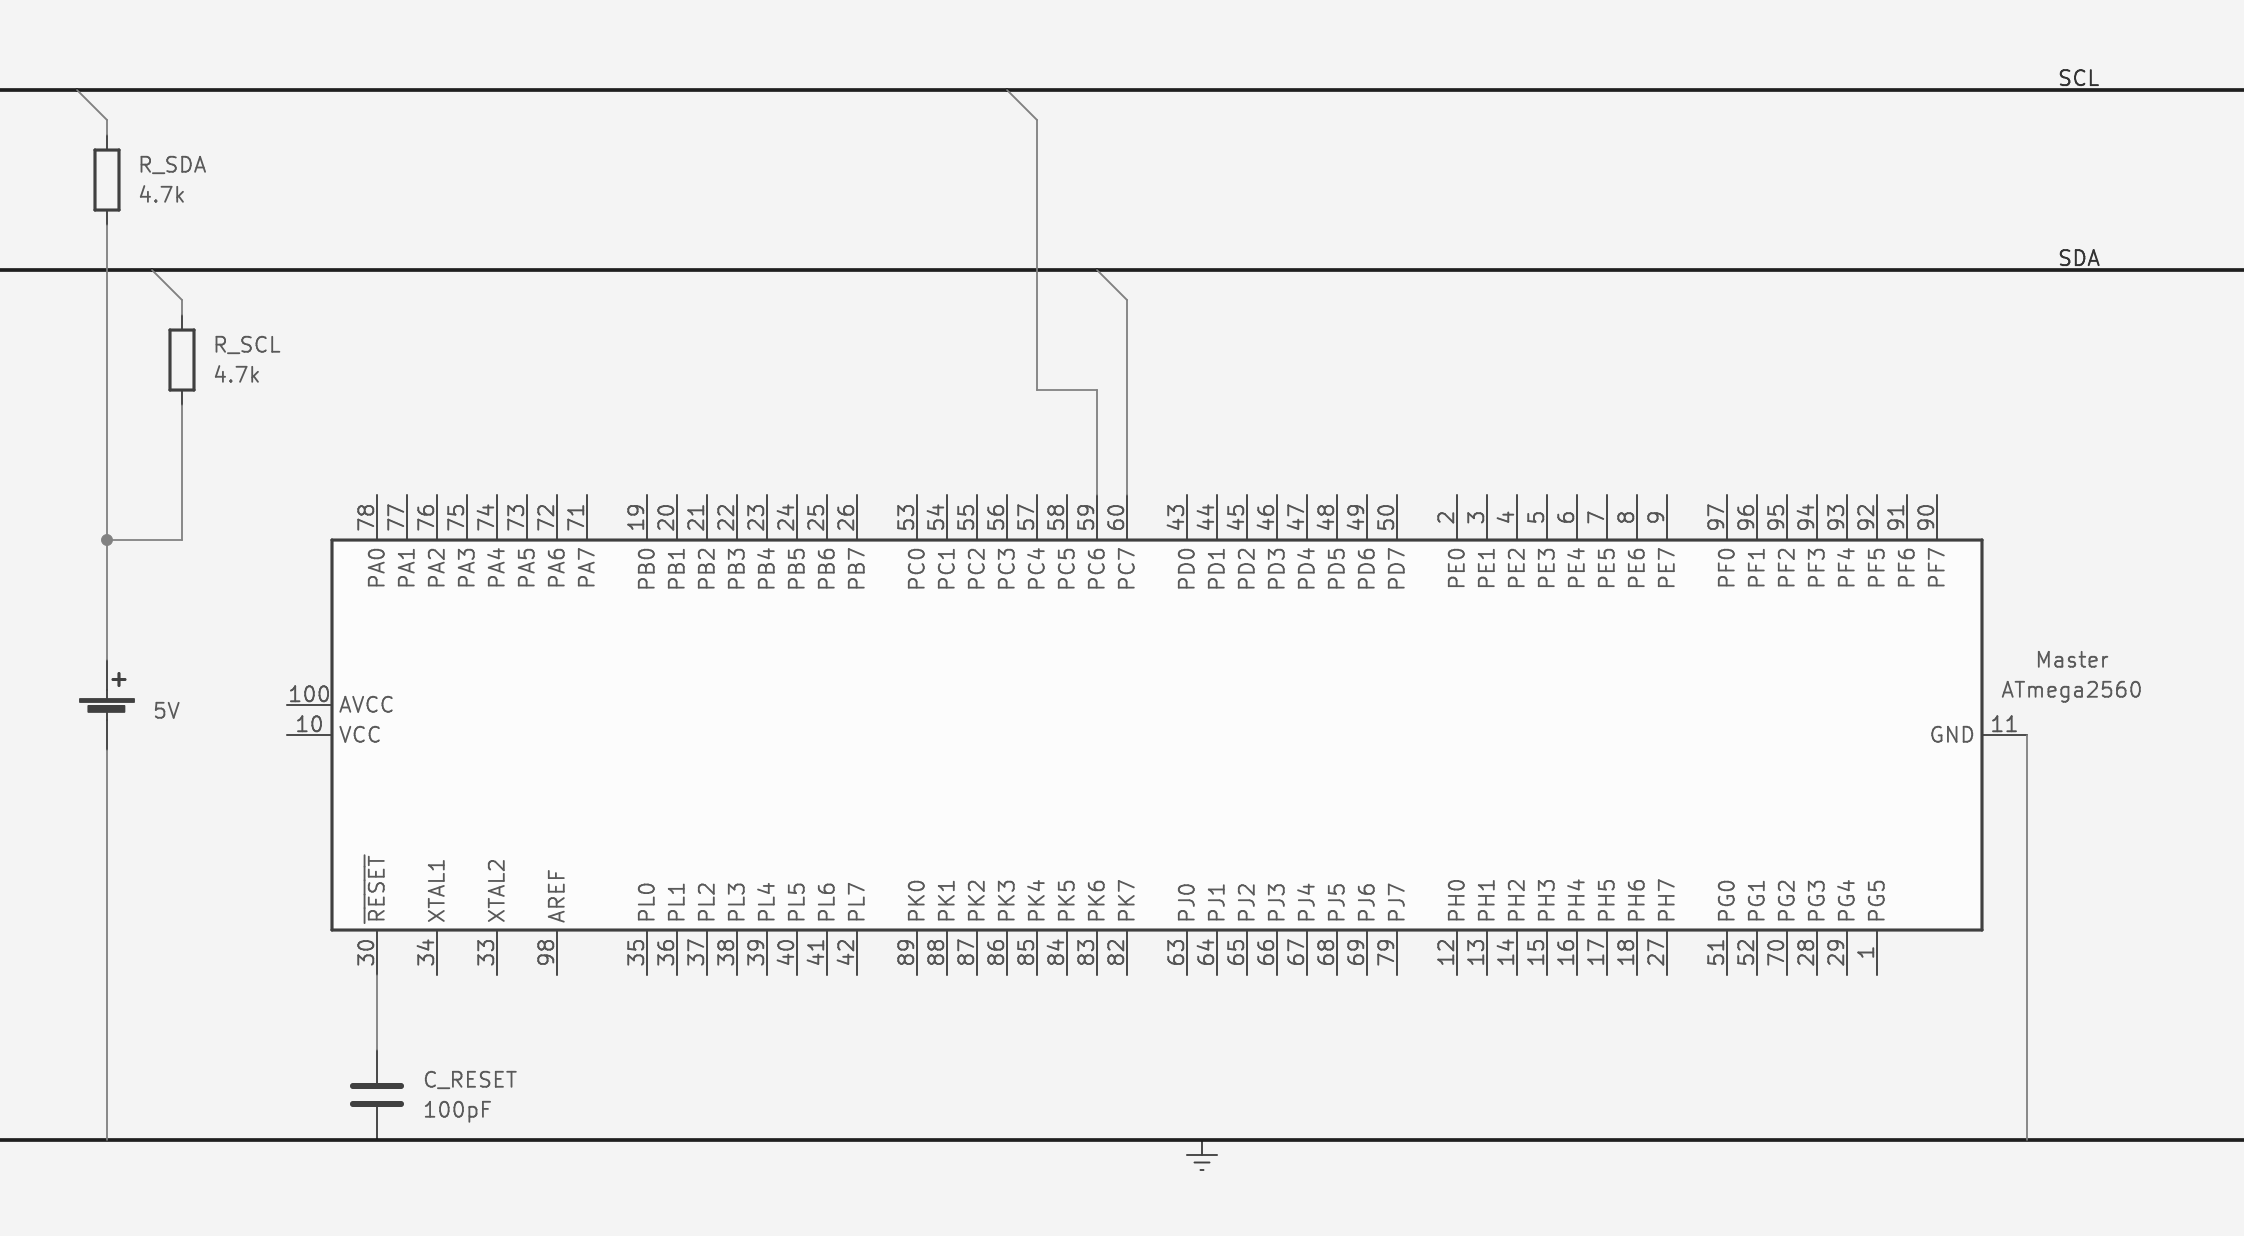
\includegraphics[width=0.9\textwidth]{../source/images/master-schematics.png}
  \caption{Master controller schematics}
\end{figure}
\end{frame}

\begin{frame}{Software modules}
\begin{figure}
  \centering
  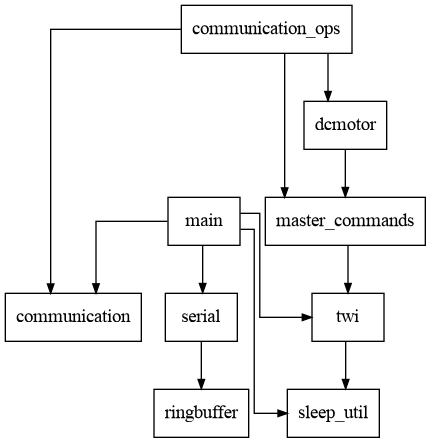
\includegraphics[width=0.5\textwidth]{../source/images/master-deps.png}
  \caption{Master controller firmware modules dependency graph}
\end{figure}
\end{frame}

\hypertarget{slave-controller}{%
\section{Slave Controller}\label{slave-controller}}

\begin{frame}{Features}
\begin{itemize}
  \item Is itself an \textbf{ATMega2560} microcontroller unit
  \item Manages a single dc motor
  \item Communicates with the master controller using the \textbf{I2C}
    interface
  \item Execute commands issued by the master controller
  \item Embedded software-defined \textbf{Proportional-Integral-Derivative}
    controller
\end{itemize}
\end{frame}

\begin{frame}{Hardware setup}
\begin{figure}
  \centering
  \LimitedIncludeGraphics{../source/images/slave-schematics.png}
  \caption{Slave controller schematics}
\end{figure}
\end{frame}

\begin{frame}{Software modules}
\begin{figure}
  \centering
  \LimitedIncludeGraphics{../source/images/slave-deps.png}
  \caption{Slave controller firmware modules dependency graph}
\end{figure}
\end{frame}

\hypertarget{client-master-communication}{%
\section{Client-Master
Communication}\label{client-master-communication}}

\begin{frame}{Characteristics}
\begin{itemize}
  \item Built on top of the \textbf{serial} interface
  \item Completely binary
  \item \textbf{Packet}-based
  \item Packet integrity is checked via \textbf{CRC-8} checksum
  \item Interrupt-driven for the master controller
\end{itemize}
\end{frame}

\begin{frame}{Packets}
Each packet is composed of:

\begin{itemize}
  \item A \textbf{header} containing:
  \begin{itemize}
    \item Packet id
    \item Packet type
    \item Whole packet size
    \item DC motor selector
  \end{itemize}
  \item An eventual \textbf{body}
  \item A trailing CRC-8 \textbf{checksum}
\end{itemize}
\end{frame}

\begin{frame}{Packet types}
\begin{longtable}[]{@{}cc@{}}
\toprule
  Type & Actual value \\
\midrule
\endhead
  \texttt{COM\_TYPE\_NULL} & \texttt{0x00} \\
  \texttt{COM\_TYPE\_HND} & \texttt{0x01} \\
  \texttt{COM\_TYPE\_ACK} & \texttt{0x02} \\
  \texttt{COM\_TYPE\_NAK} & \texttt{0x03} \\
  \texttt{COM\_TYPE\_ECHO} & \texttt{0x04} \\
  \texttt{COM\_TYPE\_PING} & \texttt{0x05} \\
  \texttt{COM\_TYPE\_GET\_SPEED} & \texttt{0x06} \\
  \texttt{COM\_TYPE\_SET\_SPEED} & \texttt{0x07} \\
  \texttt{COM\_TYPE\_APPLY} & \texttt{0x08} \\
  \texttt{COM\_TYPE\_DAT} & \texttt{0x09} \\
  \texttt{COM\_TYPE\_SET\_ADDR} & \texttt{0x0A} \\
  \texttt{COM\_TYPE\_LIMIT} & \texttt{0x0B} \\
\bottomrule
\end{longtable}
\end{frame}

\hypertarget{i2c-communication}{%
\section{I2C Communication}\label{i2c-communication}}

\begin{frame}{Features}
\begin{itemize}
  \item Master-Slave architecture
  \item Completely binary
  \item \textbf{Interrupt-driven} for both master and slaves
  \item \textbf{Broadcasting} capabilities through the \emph{general-call
    address} \texttt{0x00}
  \item Follows the original Philips I2C specification (year 2000)
\end{itemize}
\end{frame}

\begin{frame}{Communication Frames}
The communication frames is composed of two parts:

\begin{itemize}
  \item A heading byte representing the master \textbf{command}
  \item An optional command \textbf{argument}
\end{itemize}

\begin{longtable}[]{@{}cc@{}}
\toprule
  Command & Code \\
\midrule
\endhead
  \texttt{CMD\_GET} & \texttt{0x00} \\
  \texttt{CMD\_SET} & \texttt{0x01} \\
  \texttt{CMD\_APPLY} & \texttt{0x02} \\
  \texttt{CMD\_PING} & \texttt{0x03} \\
  \texttt{CMD\_SET\_ADDR} & \texttt{0x04} \\
\bottomrule
\end{longtable}
\end{frame}

\end{document}
